Fotos, Office Dokumente, PDFs und andere Dateitypen enthalten in den Metadaten viele Informationen, die auf den ersten Blick nicht sichtbar sind jedoch vieles verraten k�nnen.
\begin{itemize}
\item Fotos von Digitalkameras enthalten in den EXIF-Tags eine eindeutige ID der Kamera, Zeitstempel der Aufnahmen, bei neueren Modellen auch GPS-Daten. Die IPTC-Tags k�nnen Schlagw�rter und Bildbeschreibungen der Fotoverwaltung enthalten. XMP Daten enthalten den Autor und der Comment �blicherweise die verwendete Software.
\item Office Dokumente enthalten Informationen zum Autor, letzte �nderungen, verwendete Softwareversion und vieles mehr. Diese Angaben sind auch in PDFs enthalten, die mit der Export-Funktion von OpenOffice.org oder Microsoft Office erstellt wurden.
\end{itemize}

Vor dem Upload der Dateien ins Internet ist es ratsam, diese �berfl�ssigen Informationen zu entfernen. Es gibt mehrere Firmen, die sich auf die Auswertung dieser Metadaten spezialisiert haben. Ein Beispiel ist die Firma Heypic, die die Fotos von Twitter durchsucht und anhand der GPS-Koordinaten auf einer Karte darstellt. Auch Strafverfolger nutzen diese Informationen. Das FBI konnte einen Hacker mit den GPS-Koordinaten im Foto seiner Freundin finden\footnote{ \href{http://www.tech-review.de/include.php?path=content/news.php\&contentid=14968}{http://www.tech-review.de/include.php?path=content/news.php\&contentid=14968}}.\\

Der \textit{StolenCameraFinder}\footnote{ \href{http://www.stolencamerafinder.com}{http://www.stolencamerafinder.com}} sucht anhand der Kamera ID in den EXIF-Tags alle Fotos, die mit dieser Kamera gemacht wurden. Da die Kamera ID mit hoher Wahrscheinlichkeit eindeutig einer Person zugeordnet werden kann, sind viele Anwendungen f�r diese Suche denkbar.

\section{Fotos und Bilddateien anonymisieren}
\begin{itemize}
\item \textbf{Irfan View} \footnote{ \href{http://www.heise.de/download/irfanview.html}{http://www.heise.de/download/irfanview.html}} (Windows) kann in Fotos mit \textit{�ffnen} und \textit{Speichern} die Metatags entfernen. Im Batchmode kann man die Funktion \textit{Konvertieren} nutzen, um mehrere Bilder mit einem Durchgang zu bearbeiten. Man konvertiert die Fotos von JPEG nach JPEG und gibt dabei in den Optionen an, dass keine EXIF, XMP und IPTC Daten erhalten bleiben sollen.

\begin{figure}[htb]
\begin{center}
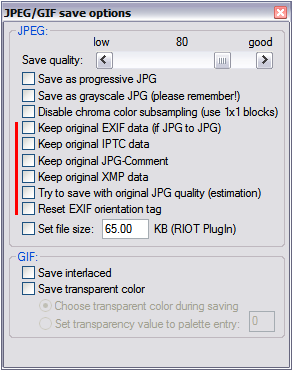
\includegraphics[scale=0.6]{../screenshots/irfan1.png}
\caption{Informationen in Fotos l�schen mit Irfan View}
\label{abb:irfanview}
\end{center}
\end{figure}

 \item \textbf{exiv2} (f�r Linux) ist ein nettes kleines Tool zum Bearbeiten von EXIF, XMP und IPTC Informationen in Bilddateien. Es ist in den meisten Linux Distributionen enthalten. Nach der Installation kann man z.B. Fotos auf der Kommandozeile s�ubern: 

\begin{verbatim}
   > exiv2 rm foto.jpg
\end{verbatim}
\end{itemize}

\section{PDF-Dokumente s�ubern}
F�r Windows gibt es das Tool \textbf{BeCyPDFMetaEdit} \footnote{ \href{http://www.becyhome.de/download\_ger.htm}{http://www.becyhome.de/download\_ger.htm}} in einer portablen Version f�r den USB-Stick oder als Installer. Nach dem Download und evtl. der Installation kann man das Tool starten und die zu s�ubernden PDF-Dokumente laden. Auf den Reitern \textit{Metadaten} und \textit{Metadaten (XMP)} klickt man auf den Button \textit{Alle Felder l�schen} und speichert das ges�uberte Dokument.

\begin{figure}[htb]
\begin{center}
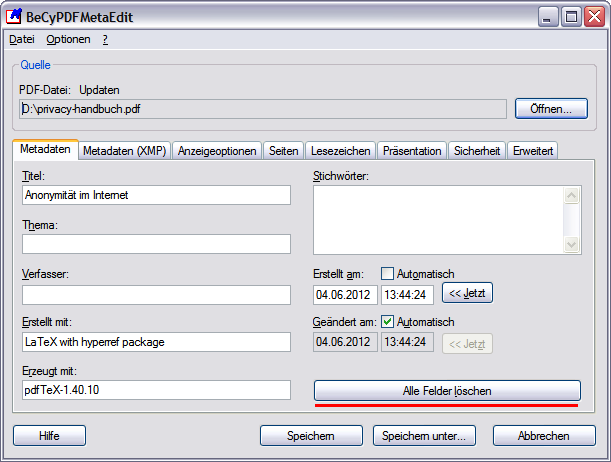
\includegraphics[scale=0.6]{../screenshots/becypdfedit.png}
\caption{Metadaten in PDF-Dokumenten l�schen}
\label{abb:irfanview}
\end{center}
\end{figure}